\documentclass{beamer}
\usepackage[utf8]{inputenc}

\usetheme{Madrid}
\usecolortheme{default}
\usepackage{amsmath,amssymb,amsfonts,amsthm}
\usepackage{txfonts}
\usepackage{tkz-euclide}
\usepackage{listings}
\usepackage{adjustbox}
\usepackage{array}
\usepackage{tabularx}
\usepackage{gvv}
\usepackage{lmodern}
\usepackage{circuitikz}
\usepackage{tikz}
\usepackage{graphicx}
\setbeamertemplate{page number in head/foot}[totalframenumber]
\usepackage[T1]{fontenc}
\usepackage{tcolorbox}
\tcbuselibrary{minted,breakable,xparse,skins}

\definecolor{bg}{gray}{0.95}
\DeclareTCBListing{mintedbox}{O{}m!O{}}{%
  breakable=true,
  listing engine=minted,
  listing only,
  minted language=#2,
  minted style=default,
  minted options={%
    linenos,
    gobble=0,
    breaklines=true,
    breakafter=,,
    fontsize=\small,
    numbersep=8pt,
    #1},
  boxsep=0pt,
  left skip=0pt,
  right skip=0pt,
  left=25pt,
  right=0pt,
  top=3pt,
  bottom=3pt,
  arc=5pt,
  leftrule=0pt,
  rightrule=0pt,
  bottomrule=2pt,
  toprule=2pt,
  colback=bg,
  colframe=orange!70,
  enhanced,
  overlay={%
    \begin{tcbclipinterior}
    \fill[orange!20!white] (frame.south west) rectangle ([xshift=20pt]frame.north west);
    \end{tcbclipinterior}},
  #3,
}

% Code style
\lstset{
    language=C,
    basicstyle=\ttfamily\small,
    keywordstyle=\color{blue},
    stringstyle=\color{orange},
    commentstyle=\color{green!60!black},
    numbers=left,
    numberstyle=\tiny\color{gray},
    breaklines=true,
    showstringspaces=false,
}

% Title info
\title %optional
{4.2.16}
\date{October 2, 2025}
\author % (optional)
{EE25BTECH11018 - Darisy Sreetej}

\begin{document}

\frame{\titlepage}

\begin{frame}{Question}
Point $\vec{P}(0, 2)$ is the point of intersection of the y-axis and the perpendicular bisector of the line segment joining the points $\vec{A}(-1,1)$ and $\vec{B}(3,3).$\\
\textbf{True} or \textbf{False}
\end{frame}
\begin{frame}
    \begin{table}[H]
	\centering
	\caption{}
	\begin{tabular}{|c|c|}
\hline
\textbf{Variable} & \textbf{Value} \\
\hline
$A$ & $(0,-\frac{3}{2})$ \\
\hline
$m$ & $\frac{1}{2}$ \\
\hline
\end{tabular}
	\label{}
\end{table}
\end{frame}
\begin{frame}{Obtaining the perpendicular bisector}
Let the equation of perpendicular bisector be
\begin{align}
	\vec{n}^\top\vec{x}=C
\end{align}
Let $\vec{R}$ be the midpoint of the line segment $\vec{AB}$
\begin{align}
    \vec{R}=\frac{\vec{A}+\vec{B}}{2} = \frac{\myvec{-1\\1}+\myvec{3\\3}}{2}
\end{align}
\begin{align}
    \vec{R}=\myvec{1\\2}
\end{align}
The direction vector of $\vec{AB}$ is 
\begin{align}
	\vec{n}=\vec{B}-\vec{A}=\myvec{4\\2}
\end{align}
\end{frame}
\begin{frame}
As it passes through the midpoint $\vec{R}$ ,
\begin{align}
\myvec{4&2}\myvec{1\\2}=C
\end{align}
\begin{align}
	C=8
\end{align}
Therefore , the equation of the perpendicular bisector is 
\begin{align}
	\myvec{4\\2}^\top\vec{x}=8
\end{align}
\begin{align}
	\myvec{2\\1}^\top\vec{x}=4
\end{align}
\end{frame}
\begin{frame}{Obtaining point of intersection}
Let $\vec{P}$ be the point of intersection of y-axis with the perpendicular bisector \\
Intersection with y-axis $(x=0)$ ,
\begin{align}
    \myvec{2&1}\myvec{0\\y}=4
\end{align}
\begin{align}
	y=4
\end{align}
Thus,
\begin{align}
	P=\myvec{0\\4}
\end{align}
The point of intersection is $P(0,4)$ \\
\end{frame}
\begin{frame}{Conclusion}
Therefore the Statement is \textbf{False}
\end{frame}
\begin{frame}{Plot}
    \centering
    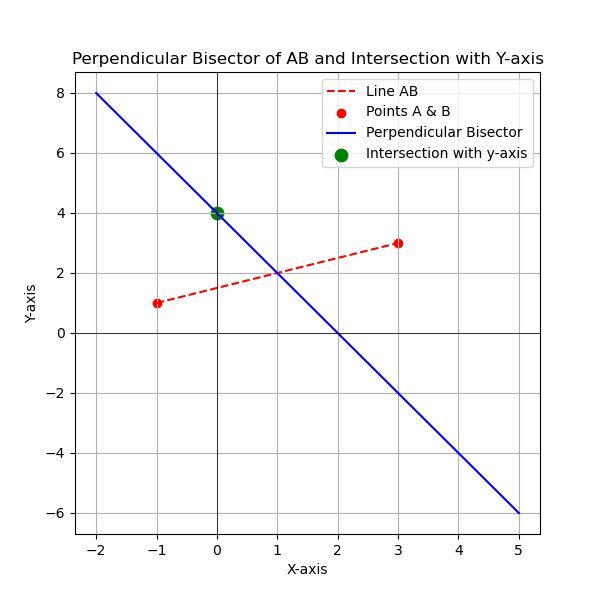
\includegraphics[width=3\columnwidth, height=0.8\textheight, keepaspectratio]{figs/fig.png}     
\end{frame}

\begin{frame}[fragile]
\frametitle{C code}
    \begin{lstlisting}[language=C]
#include <stdio.h>

// Function to calculate midpoint of AB
void midpoint(float Ax, float Ay, float Bx, float By, float *Mx, float *My) {
    *Mx = (Ax + Bx) / 2.0;
    *My = (Ay + By) / 2.0;
}

// Function to calculate direction vector (B - A)
void direction(float Ax, float Ay, float Bx, float By, float *dx, float *dy) {
    *dx = Bx - Ax;
    *dy = By - Ay;
}

// Function to calculate perpendicular bisector equation coefficients
\end{lstlisting}
\end{frame}
\begin{frame}[fragile]
    \frametitle{C Code }
    \begin{lstlisting}[language=C]
// Returns c value; coeff[0] = a, coeff[1] = b
float perpendicularBisector(float Ax, float Ay, float Bx, float By, float coeff[2]) {
    float Mx, My, dx, dy;

    midpoint(Ax, Ay, Bx, By, &Mx, &My);
    direction(Ax, Ay, Bx, By, &dx, &dy);
    coeff[0] = dx;
    coeff[1] = dy;
    return (coeff[0] * Mx + coeff[1] * My);
}

// Function to find intersection with y-axis (x = 0)
float intersectionY(float coeff[2], float c) {
    // Equation: a*0 + b*y = c → y = c/b
    return c / coeff[1];
}
     \end{lstlisting}
\end{frame}
\begin{frame}[fragile]
    \frametitle{Python + C Code }
    \begin{lstlisting}[language=Python]
import ctypes
import matplotlib.pyplot as plt
import numpy as np

# Load the shared library
lib = ctypes.CDLL("./perpendicular.so")

# Argument and return types
lib.perpendicularBisector.argtypes = [ctypes.c_float, ctypes.c_float,
                                      ctypes.c_float, ctypes.c_float,
                                      ctypes.POINTER(ctypes.c_float)]
lib.perpendicularBisector.restype = ctypes.c_float

    \end{lstlisting}
\end{frame}

\begin{frame}[fragile]
    \frametitle{Python + C code}

    \begin{lstlisting}[language=Python]
lib.intersectionY.argtypes = [ctypes.POINTER(ctypes.c_float), ctypes.c_float]
lib.intersectionY.restype = ctypes.c_float

# Input points
Ax, Ay = -1.0, 1.0
Bx, By = 3.0, 3.0

# Prepare coeff array (a,b)
coeff = (ctypes.c_float * 2)()
c = lib.perpendicularBisector(Ax, Ay, Bx, By, coeff)

a, b = coeff[0], coeff[1]
print(f"Equation: {a:.1f}x + {b:.1f}y = {c:.1f}")

# Intersection with y-axis
y_inter = lib.intersectionY(coeff, c)
print(f"Intersection with y-axis: (0, {y_inter:.1f})")
    \end{lstlisting}
\end{frame}

\begin{frame}[fragile]
    \frametitle{Python + C code}

    \begin{lstlisting}[language=Python]
# Plotting
# Original line AB
x_vals = np.array([Ax, Bx])
y_vals = np.array([Ay, By])

# Perpendicular bisector line: ax + by = c  -> y = (c - a*x)/b
x_line = np.linspace(-2, 5, 100)
y_line = (c - a * x_line) / b

plt.figure(figsize=(6,6))
plt.plot(x_vals, y_vals, 'r--', label="Line AB")
plt.scatter([Ax, Bx], [Ay, By], color='red', label="Points A & B")

plt.plot(x_line, y_line, 'b-', label="Perpendicular Bisector")
plt.scatter([0], [y_inter], color='green', s=80, label="Intersection with y-axis")

plt.axhline(0, color='black', linewidth=0.5)
    \end{lstlisting}
\end{frame}
\begin{frame}[fragile]
    \frametitle{Python + C code}

    \begin{lstlisting}[language=Python]
plt.axvline(0, color='black', linewidth=0.5)

plt.legend()
plt.grid(True)
plt.xlabel("X-axis")
plt.ylabel("Y-axis")
plt.title("Perpendicular Bisector of AB and Intersection with Y-axis")
plt.show()
      \end{lstlisting}
\end{frame}
\begin{frame}[fragile]
    \frametitle{Python code}
    \begin{lstlisting}[language=Python]
import matplotlib.pyplot as plt
import numpy as np

# Input points
Ax, Ay = -1, 1
Bx, By = 3, 3

# Midpoint
Mx, My = (Ax + Bx) / 2, (Ay + By) / 2

# Direction vector of AB
dx, dy = Bx - Ax, By - Ay

# Equation of perpendicular bisector: a*x + b*y = c
a, b = dx, dy
c = a*Mx + b*My

# Intersection with y-axis (x=0)
y_inter = c / b

    \end{lstlisting}
\end{frame}

\begin{frame}[fragile]
    \frametitle{Python code}

    \begin{lstlisting}[language=Python]
print(f"Equation of perpendicular bisector: {a}x + {b}y = {c}")
print(f"Intersection with y-axis: (0, {y_inter})")

# Line AB
x_AB = [Ax, Bx]
y_AB = [Ay, By]

# Perpendicular bisector line
x_line = np.linspace(-2, 5, 100)
y_line = (c - a*x_line) / b

plt.figure(figsize=(6,6))
plt.plot(x_AB, y_AB, 'r--', label="Line AB")
plt.scatter([Ax, Bx], [Ay, By], color='red', label="Points A & B")

plt.plot(x_line, y_line, 'b-', label="Perpendicular Bisector")
plt.scatter([0], [y_inter], color='green', s=80, label="Intersection with y-axis")
           \end{lstlisting}
\end{frame}
\begin{frame}[fragile]
    \frametitle{Python code}

    \begin{lstlisting}[language=Python]
plt.axhline(0, color='black', linewidth=0.5)
plt.axvline(0, color='black', linewidth=0.5)

plt.legend()
plt.grid(True)
plt.xlabel("X-axis")
plt.ylabel("Y-axis")
plt.title("Perpendicular Bisector of AB and Intersection with Y-axis")
plt.show()

    \end{lstlisting}
\end{frame}
\end{document}
